\section{Fourierreihen periodischer Funktionen}
	\subsection{Bausteine}
		\textbf{Idee:}\\[3pt]
		$T$-Periodische, mit Limes stückweise stetigen Funktionen, durch Aufsummieren ebenfalls periodischer Basisfunktionen
		(sin, cos) zu approximieren.\\[3pt]

		\textbf{Basisfunktionen:}\\[3pt]
		\begin{minipage}[t]{0.5\textwidth}
			\begin{tabular}{llll}
				Konstante: & $cos(0 \cdot \omega_{f} t) = 1$ & &\\[3pt]
				$1 \times$ Frequenz $f$  & $\cos(1 \cdot \omega_{f} t)$ & ; & $\sin(1 \cdot \omega_{f} t)$\\[3pt]
				$2 \times$ Frequenz $f$: & $\cos(2 \cdot \omega_{f} t)$ & ; & $\sin(2 \cdot \omega_{f} t)$\\[3pt]
				$3 \times$ Frequenz $f$: & $\cos(3 \cdot \omega_{f} t)$ & ; & $\sin(3 \cdot \omega_{f} t)$\\[3pt]
				usw. & & &\\[3pt]
			\end{tabular}
		\end{minipage}
		\begin{minipage}[t]{0.2\textwidth}
			
		\end{minipage}
		\begin{minipage}[t]{0.3\textwidth}
			\fbox{
				\begin{tabular}{ll}
					Frequenz: & $f = \dfrac{1}{T}$\\[7pt]
					Kreisfrequenz: & $\omega_f = 2 \pi f$\\[3pt]
					Periodendauer: & $T = \dfrac{2 \pi}{\omega_f} = \dfrac{1}{f}$\\[6pt]
					Nullphasenwinkel: & $\varphi$\\[6pt]
				\end{tabular}
			}
		\end{minipage}
	
	\subsection{Berechnung der Fourierkoeffizienten (in $\mathbb{R}$)}
		\textbf{Die Funktion $f(t)$ soll durch folgende Linearkombination dargestellt werden:}\\[3pt]
		\fbox{$FR[f(t)] = \dfrac{a_0}{2} + \sum\limits_{n=1}^{\infty} [a_n \cdot \cos(n \omega_f t) + b_n \sin(n \omega_f t)]$}\\[3pt]
		\begin{minipage}[t]{0.5\textwidth}
			\textbf{Berechnung von $a_0$, $a_n$ und $b_n$\\[1pt] (Fourierkoeffizienten):}\\[3pt]
			\begin{tabular}{|lll|l|}
				\hline
				$\displaystyle a_0$ & $=$ & $\displaystyle \dfrac{2}{T} \cdot \int\limits_{0}^{T} f(t) dt$ & $\displaystyle n = 0$\\[0.2pt]
				\hline
				$\displaystyle b_0$ & $\displaystyle =$ & $\displaystyle 0$ & $\displaystyle n = 0$\\
				\hline
				$\displaystyle a_n$ & $\displaystyle =$ & $\displaystyle \dfrac{2}{T} \cdot \int\limits_{0}^{T} f(t) \cdot \cos(n \omega_f t) dt$ & $\displaystyle n = 0, 1, 2, \cdots$\\
				\hline
				$\displaystyle b_n$ & $\displaystyle =$ & $\displaystyle \dfrac{2}{T} \cdot \int\limits_{0}^{T} f(t) \cdot \cos(n \omega_f t) dt$ & $\displaystyle n = 1, 2, 3, \cdots$\\
				\hline
			\end{tabular}
		\end{minipage}
		\begin{minipage}[t]{0.5\textwidth}
			\textbf{Orthogonalitätsbeziehungen:\\[1pt]}\\[3pt]
			\begin{tabular}{|l|}
				\hline
				$\displaystyle \int\limits_{0}^{T} \cos(m \omega_f t) \cdot \cos(n \omega_f t) dt = \left\lbrace 
					\begin{array}{ll}
						T & \text{für: } m = n = 0\\
						\dfrac{T}{2} & \text{für: } m = n > 0\\
						0 & \text{für: } m \neq n\\
					\end{array} \right.$\\[3pt]
				$\displaystyle \int\limits_{0}^{T} \sin(m \omega_f t) \cdot \sin(n \omega_f t) dt = \left\lbrace 
					\begin{array}{ll}
						\dfrac{T}{2} & \text{für: } m = n > 0\\
						0 & \text{für: } m \neq n\\
					\end{array} \right.$\\[3pt]
				$\displaystyle \int\limits_{0}^{T} \sin(m \omega_f t) \cdot \sin(n \omega_f t) dt = 0$\\[3pt]
				\hline
			\end{tabular}
		\end{minipage}
	
	\subsection{Sätze zur Berechnung der Fourierkoeffizienten}
		\subsubsection{Symmetrie}
			\begin{minipage}[]{0.5\textwidth}
				\begin{tabular}{|c|c|}
					\hline
					\textbf{Gerade Funktion} & \textbf{Ungerade Funktion}\\[3pt]
					\hline
					\scalebox{0.45}{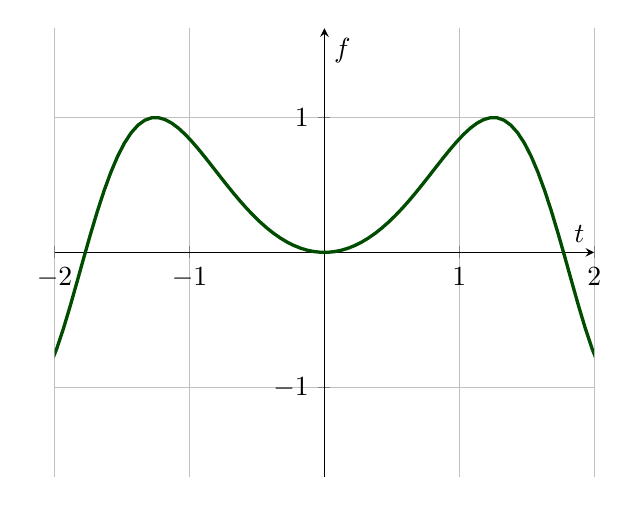
\begin{tikzpicture}
	\begin{axis}[axis lines=middle, axis equal, grid=both, xmin = -2, xmax = 2, ymin = -1, ymax = 1, xlabel = $t$, ylabel = $\operatorname{f}$]
		\addplot[black!70!green, very thick, samples = 200] {sin(deg(x^2))} node[above, red] at (10, 10) {$f$};
	\end{axis}
\end{tikzpicture}} & \scalebox{0.45}{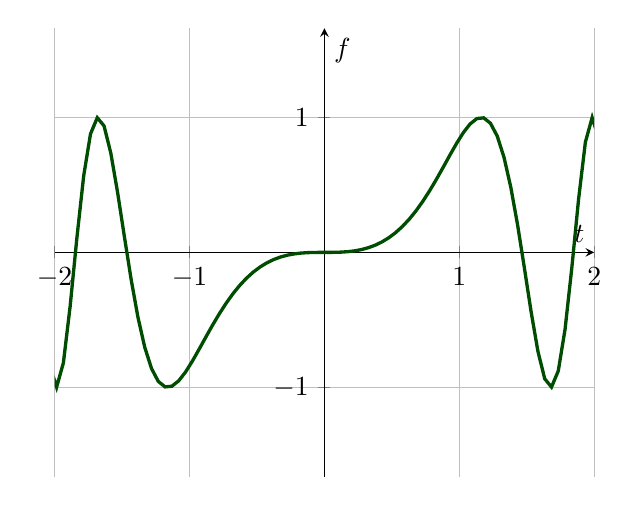
\begin{tikzpicture}
	\begin{axis}[axis lines=middle, axis equal, grid=both, xmin = -2, xmax = 2, ymin = -1, ymax = 1, xlabel = $t$, ylabel = $\operatorname{f}$]
		\addplot[black!70!green, very thick, samples = 200] {sin(deg(x^3))} node[above, red] at (100, 100) {$f$};
	\end{axis}
\end{tikzpicture}}\\[3pt]
					\hline
					achsensymmetrisch & punktsymmetrisch\\[3pt]
					$\displaystyle f(t) = f(-t)$ & $f(t) = -f(-t)$\\[3pt]
					\hline
					Beispiel: $\displaystyle \cos$ & Beispiel: $\sin$\\[3pt]
					\hline
					$\displaystyle \int\limits_{0}^{T} f(t) dt = 2 \int\limits_{0}^{T/2} f(t) dt$ & $\displaystyle \int\limits_{0}^{T} f(t) dt = 0$\\[3pt]
					\hline
				\end{tabular}
			\end{minipage}
			\begin{minipage}[]{0.5\textwidth}
				\textbf{Rechnen mit geraden und ungeraden Funktionen:}\\[3pt]
				\begin{tabular}{|lclcl|}
					\hline
					gerade & $\cdot$ & gerade & $=$ & gerade\\[3pt]
					ungerade & $\cdot$ & ungerade & $=$ & gerade\\[3pt]
					gerade & $\cdot$ & ungerade & $=$ & ungerade\\[3pt]
					\hline
				\end{tabular}\\[3pt]
				\textbf{Fourierkoeffizienten $a_n$, $b_n$:}\\[3pt]
				\begin{tabular}{|l|ll|}
					\hline
					$f(t)$		&  $a_n$, $b_n$ & \\[3pt]
					\hline
					gerade		& $b_n = 0$ ; & $\displaystyle a_n = \dfrac{4}{T} \int\limits_{0}^{T/2} f(t) \cdot \cos(n \omega_f t) dt$\\[3pt]
					\hline
					ungerade	& $a_n = 0$ ; & $\displaystyle b_n = \dfrac{4}{T} \int\limits_{0}^{T/2} f(t) \cdot \sin(n \omega_f t) dt$\\[3pt]
					\hline
				\end{tabular}
			\end{minipage}
		\subsubsection{Linearität}
			$f(t)$, $g(t)$ und $h(t)$ sind $T$-periodische Funktionen.\\[3pt]
			\begin{tabular}{lllll}
				Wenn gilt: 
				&
				\fbox{$h(t) = r \cdot f(t) + s \cdot g(t)$} 
				&
				$\Rightarrow$ 
				&
				\begin{tabular}{l}
					\fbox{$a_n^{(h)} = r \cdot a_n^{(f)} + s \cdot a_n^{(g)}$}\\[3pt]
					\fbox{$b_n^{(h)} = r \cdot b_n^{(f)} + s \cdot b_n^{(g)}$}\\[3pt]
				\end{tabular}
				&
				$r$, $s \in \mathbb{R}$
			\end{tabular}
		\subsubsection{Streckung / Stauchung}
			$f(t)$ ist eine $T$-periodische Funktion und $g(t)$ eine $\dfrac{T}{r}$-periodische Funktion.\\[3pt]
			\begin{tabular}{llllllll}
				$\Rightarrow$ 
				&
				\fbox{$g(t) = f(r \cdot t)$} 
				&
				$\Rightarrow$ 
				&
				\begin{tabular}{l}
					\fbox{$a_n^{(g)} = a_n^{(f)}$}\\[3pt]
					\fbox{$b_n^{(g)} = b_n^{(f)}$}\\[3pt]
				\end{tabular} 
				&
				$0 < r \in \mathbb{R}$
				&
				$\Rightarrow \left\lbrace 
					\begin{array}{l}
						r < 1 \rightarrow \text{Streckung}\\[3pt]
						r > 1 \rightarrow \text{Streckung}\\[3pt]
					\end{array}\right.$
				&
				und
				&
				\fbox{$\omega_g = \dfrac{2 \pi r}{T} = \omega_f \cdot r$}
			\end{tabular}
		\subsubsection{Verschiebung}
			$g(t)$ ist eine von $f(t)$ um $t_0$ verschobene T-periodische Funktion 
			$\Rightarrow \left\lbrace 
				\begin{array}{l}
					f(t + t_0) \rightarrow \text{Verschiebung nach links}\\[3pt]
					f(t - t_0) \rightarrow \text{Verschiebung nach rechts}\\[3pt]
				\end{array} 
			\right.$\\[3pt]
			\begin{tabular}{llllll}
				$\Rightarrow$
				&
				\fbox{$g(t) = f(t + t_0)$}
				&$\Rightarrow$
				&\begin{tabular}{l}
					\fbox{$a_n^{(g)} = \cos(n \omega_f t_0) \cdot a_n^{(f)} + \sin(n \omega_f t_0) \cdot b_n^{(f)}$}\\[6pt]
					\fbox{$b_n^{(g)} = -\sin(n \omega_f t_0) \cdot a_n^{(f)} + \cos(n \omega_f t_0) \cdot b_n^{(f)}$}\\[3pt]
				\end{tabular}
				&
				;
				&
				\fbox{$b_0 = 0$}\\[3pt]
			\end{tabular}
		
		\subsection{Konvergenz der Fourierreihen}
			\subsubsection{Optimalität der Fourierreihe (Approximation)}
				\begin{minipage}[b]{0.55\textwidth}
					\textbf{Abstand zwischen zwei Funktionen $f$ und $g$:}\\[3pt]
					\fbox{$\displaystyle||f - g|| = \sqrt{\dfrac{2}{T} \int\limits_{0}^{T} \left[ f(t) - g(t) \right]^2 dt}$}\\[3pt]
					Abstand $||f - g||$ zweier Funktionen kann klein sein, obschon sich die Funktionswerte stellenweise stark unterscheiden!
				\end{minipage}
				\begin{minipage}[]{0.45\textwidth}
					\scalebox{0.8}{\begin{tikzpicture}
	\begin{axis}[axis lines=middle, axis equal, grid=both, xmin=0, xmax=1, ymin=-2.5, ymax=1, xlabel = $t$, ylabel = $\operatorname{A}$]
		\addplot[name path=f, purple, very thick, samples=200] {sin(deg(x^2))} node[above, purple] at (180, 300) {$f$};
		\addplot[name path=g, cyan, very thick, samples=200] {sin(deg(2*x))*x} node[above, cyan] at (130, 280) {$g$};
		\addplot[orange!50] fill between[of=f and g];
	\end{axis}
\end{tikzpicture}}\\[3pt]
				\end{minipage}
				\textbf{Qualität der Approximation mit endlicher Fourierreihe:}\\[3pt]
				Die abbrechende Fourierreihe $s_m(t)$ approximiert $f$ hinsichtlich des Abstandes am besten!\\[3pt]
				\begin{tabular}{|lll|}
					\hline
					$\Rightarrow \quad \displaystyle ||s_m(t) - f(t)|| = ||\dfrac{a_0}{2} + \sum\limits_{n=1}^{m} [a_n \cdot \cos(n \omega_f t) + b_n \cdot \sin(n \omega_f t)] - f(t)||$ & $\rightarrow$ & wird minimal!\\[3pt]
					\textbf{Es gilt sogar:} & &\\[3pt]
					$\displaystyle \lim_{n \to \infty} ||\dfrac{a_0}{2} + \sum\limits_{n=1}^{m} [a_n \cdot \cos(n \omega_f t) + b_n \cdot \sin(n \omega_f t)] - f(t)|| = 0$ & &\\[3pt]
					\hline
				\end{tabular}\\[3pt]
				\begin{minipage}[t]{0.5\textwidth}
					\textbf{Parseval’sche Gleichung:}\\[3pt]
					\fbox{$\dfrac{a_0^2}{2} + \sum\limits_{n=1}^{m} ()a_n^2 + b_n^2) = \dfrac{2}{T} \int\limits_{0}^{T} [f(t)]^2 dt = ||f||^2$}
				\end{minipage}
				\begin{minipage}[t]{0.5\textwidth}
					\textbf{Gliedweises Differenzieren und Integrieren:}
					\begin{framed}
						Funktion $f$ ist 2-mal stetig differenzierbar\\[3pt]
						$\Rightarrow$ man darf Fourierreihe von $f$:
						\begin{itemize}
							\item[$-$] \textbf{gliedweises integrieren}
							\item[$-$] \textbf{$(k-2)$-mal gliedweise differenzieren}
				 		\end{itemize}
					\end{framed}
				\end{minipage}
				\textbf{Nullfolgen $a_n$ und $b_n$:}\\[3pt]
				Die Fourierkoeffizienten $a_n$ und $b_n$ bilden eine Nullfolge:\\[3pt]
				\fbox{$\displaystyle \lim_{n \to \infty} a_n = \lim_{n \to \infty} \dfrac{2}{T} \int\limits_{0}^{T} f(t) \cdot \cos(n \omega_f t) dt = 0$}
				\fbox{$\displaystyle \lim_{n \to \infty} b_n = \lim_{n \to \infty} \dfrac{2}{T} \int\limits_{0}^{T} f(t) \cdot \sin(n \omega_f t) dt = 0$}\\[3pt]
				$\Rightarrow$ Je häufiger $f$ stetig differenzierbar ist, desto schneller gehen $a_n$ bzw. $b_n$ gegen $0$!\\[3pt]
				\begin{minipage}[t]{0.5\textwidth}
					\fbox{$|a_n| \leq \dfrac{c}{n^{k + 1}}$}
					\fbox{$|b_n| \leq \dfrac{c}{n^{k + 1}}$}
					$\begin{array}{l}
						c \in \mathbb{R}\\
						n \in \mathbb{N}\\
					\end{array}$
				\end{minipage}
				\begin{minipage}[t]{0.5\textwidth}
					\begin{tabular}{l}
						$(k - 1)$-mal stetig differenzierbar\\
						$k$-te Ableitung stückweise mit Limes stetig, monoton\\
					\end{tabular}
				\end{minipage}
				